
\documentclass[template=tabling,81pt,headonall]{azmoon}
\usepackage{xepersian}
\usepackage{amsfonts}
\usepackage{graphicx}
\graphicspath{ {./images/} }
\settextfont{Yas}
\setdigitfont{A Iranian Sans}
\usepackage{fontawesome5}

\printanswers
    \teacher{محمد صالح علی اکبری}
    \teachertitle{دبیر}
    \city{گناباد}
    \schooltitle{متوسطه دوره دوم}
    \school{شاهد امام (ره)}
    \grade{نهم}
    \branch{-}
    \topic{ریاضی}
    \examdate{شهریور 1402}
    \answertime{120 دقیقه}
    \begin{document}
	\begin{questions}
		\nointerlineskip%
		\vskip-\baselineskip
		\question{%
متناظر با هر یک از ناحیه‌های مشخص شده روی محور، یک نابرابری بنویسید. \\ 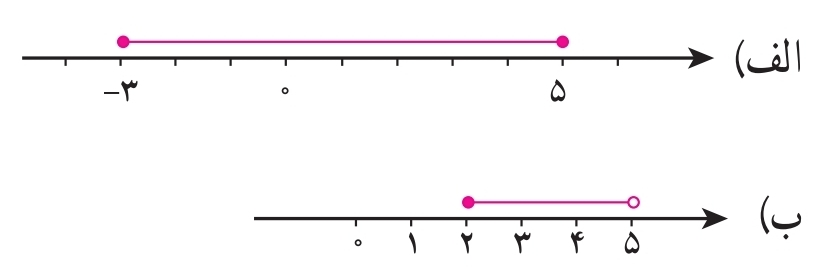
\includegraphics[scale = 0.3]{baze_mehvar_nohom}}\question{%
مجموعه جواب نامعادله‌های زیر را به دست آورید.
    \begin{LTR}
        \begin{parts}[1]\part{$2(x-3)+5<5-x$}
‌\\\part{$3-2x \geq 5(3-2x)$}
‌\\\part{$\dfrac{y-3}{4}-1>\dfrac{y}{2}$}
‌\\\part{$-2-\dfrac{q}{4} \leq \dfrac{1+q}{3}$}
\end{parts}
\end{LTR}
        ‌
\\
    }\question{%
۵ جواب برای دستگاه معادله خطی زیر بنویسید. \\ 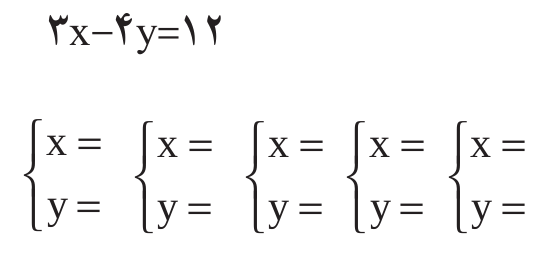
\includegraphics[scale = 0.3]{moadelekhat}}\question{%
معادلات خط زیر را رسم کنید.
    \begin{parts}[1]\part{$y = \dfrac{1}{2}x + 4$}
‌\\‌\\\part{$2y = 3 x + 7$}
‌\\‌\\\part{$4x + 3 y = 0$}
‌\\‌\\\part{$4x + 3y  - 3 = 0$}
\end{parts}
‌
\\‌
\\
    }\question{%
دستگاه معادلات زیر را حل کنید.
    \begin{LTR}
        \begin{parts}[1]\part{$x + y = 5 $ \\  $2 x + y = 8$}
‌\\‌\\\part{$4 x + y = 4$ \\ $2x + 2 y = 3.5$}
‌\\‌\\\part{$3x + 3 y + z = 11 \\ 2 z + 2 x = 12 \\ 4 y + z = 5 + \dfrac{1}{3}$}
\end{parts}
\end{LTR}
        ‌
\\‌
\\
    }\question{%
دستگاه معادلات زیر را به روش رسمی حل کنید. \\ $y = x + 1$ \\ $y = -x + 3$‌
\\‌
\\‌
\\}\end{questions}
    \end{document}
    